\documentclass[xcolor=dvipsnames]{beamer}
\usetheme{CambridgeUS}
\usepackage[labelformat=simple,
labelsep=period,
font={footnotesize},     %scriptsize, footnotesize, small, normalsize
labelfont=bf,
width=0.9\textwidth,
justification=justified,
singlelinecheck=false
]{caption}
\usepackage[utf8]{inputenc}
\usepackage[spanish, es-tabla]{babel}
\usepackage{amsmath}
\usepackage{subfigure}
\usepackage{amsfonts}
\usepackage{amssymb}
\usepackage{qtree}
\usepackage{tikz}
\usepackage{pgfplots,pgfplotstable}
\usepgfplotslibrary{statistics}
\usepackage[T1]{fontenc}
\usepackage{bera}
\usepackage{pstricks-add}
\usepackage[capposition=top]{floatrow}
\usepackage{graphicx}
 \usepackage{ragged2e}
 \usepackage{float}
 \usepackage[labelformat=simple,
 labelsep=period,
 font={footnotesize},     %scriptsize, footnotesize, small, normalsize
 labelfont=bf,
 width=0.9\textwidth,
 justification=justified,
 singlelinecheck=false
 ]{caption}
 \usepackage[justification=centering]{caption}
\setbeamersize{text margin left=5pt,text margin right=25pt}
\captionsetup[figure]{labelfont={color=Brown}}
\captionsetup[table]{labelfont={color=Brown}}

%%%%%%%%%%%%%%%%%%%%%%%%%%%%%%%%%%%%%%%%%%%%%%%%%%%%%%%%
%%% PAra el diagrama de la diapostiva 10
\usepackage{smartdiagram}
\usetikzlibrary{shapes.geometric} % required in the preamble
\smartdiagramset{
	module minimum width=3cm,
	module minimum height=1cm,
	text width=4.5cm,
	circular distance=3cm,
}
%%%%%%%%%%%%%%%%%%%%%%%%%%%%%%%%%%%%%%%%%%%%%%%%%%%%%%%%%%%
\def\angle{0}
\def\radius{2}
\def\cyclelist{{"orange","blue","red","green"}}
\newcount\cyclecount \cyclecount=-1
\newcount\ind \ind=-1	

%%%%%%%%%%%%%%DATA
\begin{filecontents}{data.csv}
	dist
	1
	2
	2.5
	2
	1
	3.5
	3
	1
	3
	2
	1
	1
	0.5
	1
	1.5
	1
\end{filecontents}

	
\author[Carlos Cardona]{Carlos Cardona}
\title{Análisis Cuantitativo I}
\subtitle{Introducción y Conceptos Básicos}
\institute[URosario]{Universidad del Rosario}
\date{27 de enero de 2017}
\begin{document}
\maketitle
	
%%%%%%%%%%%%%%%%%%%%%%%% Instroducción $$$$$$$$$$$$$$$$$$$$$$$$$$$
\section{Introducción}
\begin{frame}{Introducción}
	
\begin{itemize}
\justifying
\item ¿Sobre qué trata este curso?
\begin{itemize}
\item Investigación Social.
\item Estadística.
\item Su intersección e interacción.
\end{itemize}
\end{itemize}
\end{frame}

\begin{frame}{¿Por qué este curso?}

	\begin{enumerate}
		\justifying
\item Para aquéllos no involucrados en la investigación:
\begin{itemize}
	\justifying
\item Todos los días estamos expuestos a información que requiere un conocimiento básico de estadística.(Publicidad, noticias, campañas políticas, encuestas de opinión.) 
\end{itemize}
\item Para aquéllos involucrados en la investigación:
\begin{itemize}
		\justifying
\item La estadística fortalece el proceso investigativo. En muchos escenarios provee validez a las conclusiones encontradas.
\item Permite encontrar evidencia empírica a teorías formuladas con base en información cualitativa. 
\end{itemize}
\end{enumerate}
\end{frame}


\begin{frame}{Algunas preguntas de investigación}
\begin{itemize}
	\justifying
	\item Entre algunas de las preguntas que la estadística puede ayudar a responder se encuentran:
	\begin{itemize}
		\justifying
\item ¿Qué efecto tiene la radio sobre la participación electoral de los ciudadanos?
\item ¿La forma de agricultura tradicional practicada en la era pre-industrial tiene relación con los roles de género en la actualidad?
\item ¿Existe discriminación racial en el mercado laboral?
	\end{itemize}
\end{itemize}
\end{frame}


\begin{frame}{¿Qué es la Estadística?}
\begin{itemize}
	\justifying
\item La investigación en muchos campos requiere la recolección de información con el propósito de responder, por ejemplo, si la radio tiene algún efecto sobre el comportamiento político.
\item Al final de este proceso, el investigador usualmente termina con una gran cantidad de medidas tales como la tasa participación política, la tasa de abstención, el número de estaciones de radio, etc.
\item \emph{La estadística se refiere al conjunto de procedimientos que permiten organizar, resumir, interpretar y analizar estas características.}

\end{itemize}
\end{frame}


%%%%%%%%%%%%%%%%%% CONCEPTOS BÁSICOS %%%%%%%%%%%
\section{Conceptos Básicos}

\begin{frame}{Población (1)}
\begin{itemize}
\justifying
\item La investigación empieza con una pregunta específica a un grupo de \emph{individuos}.
\item Por ejemplo, el gobierno de un país está interesado en evaluar si la introducción de la radio en sus ciudades tiene algún efecto sobre el porcentaje de abstención.
\item En este caso, el investigador estaría interesado en todas las ciudades del país.
\item Otros ejemplos serian...
\end{itemize}
\end{frame}

\begin{frame}{Población (2)}
\begin{block}{Definición}
\centering
Una población es el conjunto completo de \emph{sujetos} de interés para una pregunta de investigación en particular. La letra \emph{N} define el tamaño de la población.
\end{block}
\end{frame}

\begin{frame}{Muestra (1)}
\begin{itemize}
\justifying
\item Una población puede ser extremadamente grande (\emph{e.g.}, la población de todo el mundo.). La investigación podría ser más específica y estar interesada en la población de este salón.
\item Claramente, el tamaño de la población puede variar según como el investigador la defina. 
\item Usualmente, las poblaciones tienden a ser grandes por lo que el investigador no puede examinar cada individuo. Por tanto, los investigadores 	seleccionan un subconjunto de la población, más pequeño y manejable.
\end{itemize}
\end{frame}

\begin{frame}{Muestra (2)}
\begin{block}{Definición}
	\centering
	Una muestra es un conjunto de individuos seleccionados de la población, con el fin de representar la población en una investigación. Usualmente se utiliza la letra \emph{n} para definir el tamaño de la muestra. 
\end{block}
\end{frame}



\begin{frame}{La relación entre Población y Muestra}
\begin{center}
\smartdiagram[circular diagram:clockwise]{LA POBLACIÓN \\ Todos los individuos \\ de interés, LA MUESTRA \\ Los individuos seleccionados \\ para participar en la \\ investigación, Los resultados para la muestra \\ son generalizados a la \\ población}
\end{center}		
\end{frame}

\begin{frame}{Variables}
\begin{itemize}
\justifying
\item Típicamente, el investigador está interesado en características específicas de los individuos de la población o en factores externos que los influencian. 
\item Por ejemplo, podría estar interesado en la influencia del conflicto sobre la participación política.
\item Al cambiar los niveles de conflicto, ¿cambia también la participación política?
\item La estadística provee una manera de lidiar con la \emph{variabilidad}, ya que permite explicar la variación de una caracteríztica a partir de la variación de otras. 
\end{itemize}
\end{frame}

\begin{frame}{Variables}
	\begin{block}{Definición}
		\centering
Una variable es una característica o condición que cambia o tiene diferentes valores para \emph{individuos} en una muestra o población. 
	\end{block}
	\begin{itemize}
\justifying
\item Para demostrar cambios en las variables, es necesario realizar mediciones de las variables que se están examinando. 
\item El conjunto completo de valores se denomina base de datos. 
	\end{itemize}
\end{frame}

\begin{frame}{¿Cómo luce una base de datos?}
\begin{center}
\begin{table}[H]
	\scalebox{0.8}{
\begin{tabular}{|c|c|c|c|c|c|}\hline
Individuo & Sexo & Estado Marital & Edad & Ingreso Anual \\ \hline
1 & M & 1 & 23 & 5150000 \\
2&M&0&37&2500000 \\
3&H&1&47&685000 \\
4&M&1&61&455000 \\
5&H&1&30&2350000 \\
6&H&0&21&0 \\
7&H&1&55&3600000 \\
8&M&0&27&5250000 \\ \hline
\end{tabular}}
\end{table}
\end{center}
\end{frame}

\begin{frame}{Parámetros y Estadísticos}
	\begin{itemize}
\justifying
\item Antes, definimos población y muestra en términos de los \emph{individuos}. Sin embargo, también nos podemos referir a población o muestra de los valores de las variables.
\item Cada muestra (o población) de individuos produce una muestra (o población) de valores! 
	\end{itemize}
\begin{block}{Definición}
\centering 
Un \emph{parámetro} es un valor númerico que describe una población. Un \emph{estadístico} es un valor numérico que describe una muestra. 
\end{block}
\end{frame}

\begin{frame}{Tipos de Métodos Estadísticos}
\begin{block}{Estadística Descriptiva}
	\justifying
Es el conjunto de métodos usados para resumir, organizar y simplificar datos.
\end{block}
\begin{block}{Estadística Inferencial}
\justifying
Consiste en técnicas que permiten realizar predicciones acerca de características de una población, basadas en información en una muestra de esa población.
\end{block}
\end{frame}


	\begin{frame}
		\begin{figure}[H]
			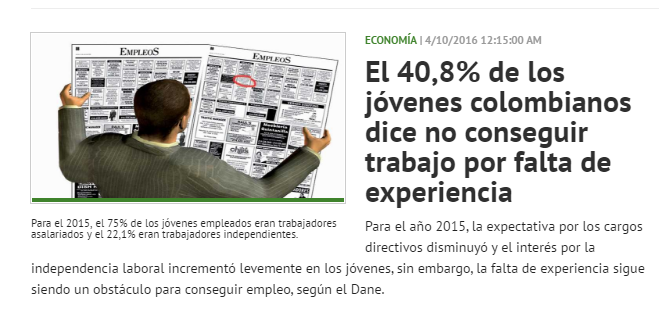
\includegraphics[width = 0.55\textwidth]{./graf4}
		\end{figure}
				\begin{figure}[H]
					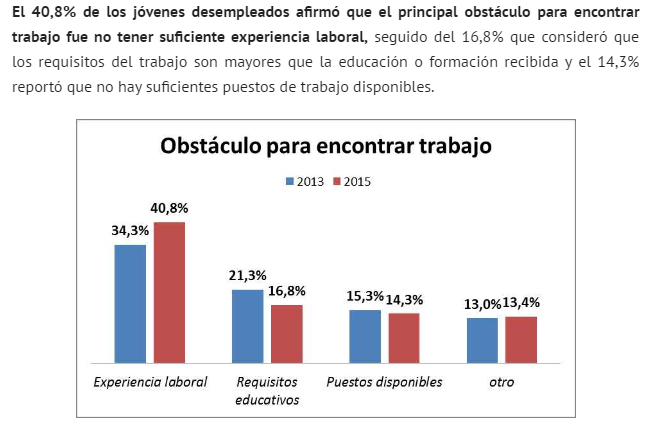
\includegraphics[width = 0.55\textwidth]{./graf5}
				\end{figure}
	\end{frame}
	
\begin{frame}{Error de Muestreo (1)}
\begin{itemize}
\justifying
\item Un problema de usar muestras, es que una muestra provee sólo información limitada de la población. 
\item A pesar de que las muestras generalmente son representativas de sus poblaciones, no se espera que una muestra de una perspectiva perfectamente precisa de la población entera. 
\item Por tanto, existe cierta discrepancia entre el estadístico muestral y el parámetro poblacional.
\end{itemize}
\end{frame}

\begin{frame}{Error de Muestreo (2)}
	\begin{block}{Definición}
		\centering
	El error de muestreo es la discrepancia, o error, que existe entre un estadístico muestral y su correspondiente parámetro poblacional.
	\end{block}
\end{frame}

\begin{frame}
		\begin{figure}[H]
			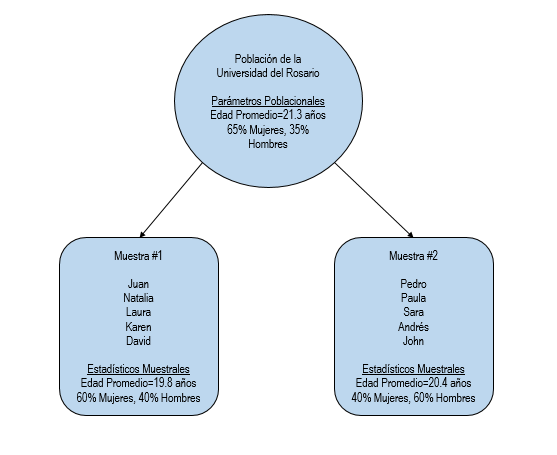
\includegraphics[width = 0.95\textwidth]{./graf6}
		\end{figure}
\end{frame}

\begin{frame}{El rol de la estadística en la investigación}
\begin{itemize}
\justifying
\item La Universidad del Rosario quiere evaluar dos métodos de estudio diferentes, para así descubrir cuál es más eficiente.
\item El propósito es demostrar si los estudiantes aprenden mejor leyendo de material impreso o de la pantalla de un computador.
\item Dos muestras son seleccionadas de la población de estudiantes de la universidad. 
\end{itemize}
\end{frame}

\begin{frame}{El rol de la estadística en la investigación}
	{\sc Paso 1: Experimento y Recolección de Datos}
		\begin{figure}[H]
			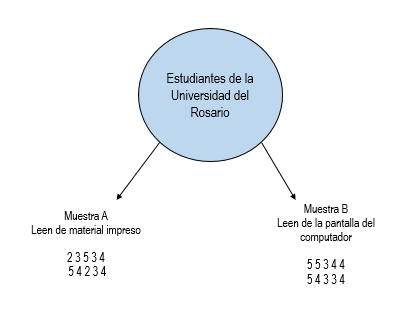
\includegraphics[width = 0.75\textwidth]{./graf7}
		\end{figure}
\end{frame}

\begin{frame}{El rol de la estadística en la investigación}
	{\sc Paso 2: Estadística Descriptiva}
	\begin{figure}[H]
		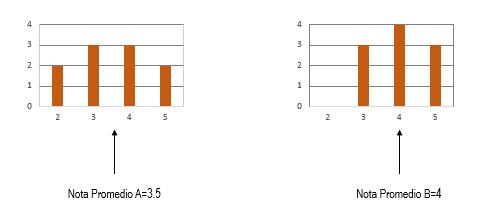
\includegraphics[width = 0.85\textwidth]{./graf8}
	\end{figure}
\end{frame}

\begin{frame}{El rol de la estadística en la investigación}
	{\sc Paso 3: Estadística Inferencial}
\begin{itemize}
\justifying
\item Los datos de la muestra presentan una diferencia de 5 décimas entre los dos métodos de estudio. Sin embargo, hay dos maneras de interpretar los resultados:
\begin{enumerate}
	\justifying
	\item Realmente no existe diferencia entre los dos métodos, y la diferencia muestral es debido al error de muestreo.
	\item Existe una diferencia entre los dos métodos, y la muestra refleja la diferencia de manera precisa. 
\end{enumerate}
\item El objetivo de la estadística inferencial es ayudar a los investigadores a decidir entre ambas interpretaciones. 
\end{itemize}
\end{frame}

\begin{frame}{Constructo}
\begin{itemize}
\justifying
\item Algunas variables como altura, peso y edad son entidades concretas y bien definidas que pueden ser observadas y medidas de manera directa.
\item Por otro lado, muchas otras variables son características internas que no pueden ser cuantificadas ni observadas directamente (\emph{e.g.}, la inteligencia, la ansiedad, la democracia, etc.).
\end{itemize}
\begin{block}{Definición}
\justifying
Un constructo es un atributo interno o característica que no puede ser directamente observada, pero es útil para describir y explicar a los \emph{individuos}.
\end{block}
\end{frame}

\begin{frame}{Definición Operacional}
\begin{itemize}
\justifying
\item Aunque los constructos son características internas no observables, es posible medir y observar atributos que son análogos de estos constructos.
\item Estos atributos externos pueden ser usados para crear una representación del constructo. Por ejemplo, el IQ para la inteligencia.
\end{itemize}
\begin{block}{Definición}
	\justifying
Una definición operacional identifica un instrumento con el cual describir un constructo interno. 
\end{block}
\end{frame}

\begin{frame}{Tipos de Variables}
{\sc Según su valor}
\begin{enumerate}
	\justifying
\item Discreta: Consiste en categorías separadas e indivisibles. No existen valores entre dos categorías vecinas.
\item Continua:  Consiste de un número infinito de posibles valores.Además, es divisible en un número infinito de partes.
\end{enumerate}
\begin{center}
\begin{table}[H]
	\caption{Algunos ejemplos}
\begin{tabular}{|c|c|}\hline
 \bfseries{Discreta} & \bfseries{Continua} \\ \hline
 Número de Hijos & Altura \\ \hline
Sexo & Nota de Clase \\ \hline
Carrera & Ingreso\\ \hline
\end{tabular}
\end{table}
\end{center}
\end{frame}

\begin{frame}{Tipos de Variables}
	{\sc Según su escala}
\begin{itemize}
\justifying
\item Escala Nominal: Consiste en un conjunto de categorías que tienen diferentes nombres.	
\begin{enumerate}
\item Estado Civil.
\item Carrera.
\end{enumerate}
\item Escala Ordinal: Consiste en un conjunto de categorías que están organizadas.
\begin{enumerate}
	\item Satisfacción con el gobierno.
	\item Estrato Socioeconómico.
\end{enumerate}
\item Escala Proporcional o de Razón: 	Consiste en valores que tienen las propiedades aritméticas.
\begin{enumerate}
	\item Ingreso laboral.
	\item Número de hijos.
\end{enumerate}
\end{itemize}
\end{frame}

\begin{frame}{Distribuciones de Frecuencias (1)}
\begin{itemize}
\justifying
\item Luego de examinar el tipo de variables que se tiene, el siguiente paso consiste en analizar cada variable por separado. 
\item ¿Cuántos sujetos caen en cada categoría o en cada valor?
\end{itemize}

\begin{block}{Definición}
\centering
Una distribución de frecuencia es una tabulación organizada del número de sujetos localizados en cada categoría en la escala de medida. 
\end{block}
\end{frame}

\begin{frame}{Distribuciones de Frecuencias (2)}
\begin{itemize}
\justifying
\item Una distribución de frecuencias puede ser estructurada como una tabla o como una gráfica.
\item Aún así, la distribución presenta los dos mismos elementos:
\begin{enumerate}
	\justifying
\item El conjunto de categorías.
\item Un registro de la frecuencia, o del número de sujetos en cada categoría.
\end{enumerate}
\item Una distribución de frecuencias presenta el panorama de cómo los valores de los sujetos se distribuyen sobre la escala de medida. 
\end{itemize}
\end{frame}

\begin{frame}{Tabla de Distribución de Frecuencias}
\begin{itemize}
\justifying
\item Supongamos que tenemos la variable X, que se define como la variable \emph{nota de un quiz de esta clase}.
\item X=\{3 3 4 5 4 4 1 4 5 3\}
\end{itemize}

\begin{center}
	\begin{table}[H]
		\caption{Distribución de Frecuencia}
		\begin{tabular}{cc} \hline
			X & \emph{f} \\ \hline
			5 & 2 \\
			4 & 4 \\
			3 & 3 \\
			1 & 1 \\ \hline
		\end{tabular}
	\end{table}
\end{center}
\begin{itemize}
	\justifying
	\item Cabe resaltar que $ \sum f = N $.
\end{itemize}
\end{frame}

\begin{frame}{Proporción y Porcentaje }
\begin{itemize}
\justifying
\item Adicional a las dos columnas básicas de la diapositiva anterior, hay otras medidas que describen la distribución de una variable.
\item Las dos más comunes son la proporción y el porcentaje. 
\item La proporción mide la fración del total del grupo que está asociado a ese valor. 

$$ p=\dfrac{f}{N}$$
\item El porcentaje es la proporción multiplicada por 100. Su interpretación es la más sencila, por tanto, es la más presentada en las tablas de distribución.

$$porcentaje=p*100=\dfrac{f}{N}*100$$
\end{itemize}
\end{frame}

\begin{frame}
\begin{itemize}
\justifying
\item Al añadirle estas dos últimas medidas, la tabla 2 queda de la siguiente manera:
\end{itemize}
\begin{center}
	\begin{table}[H]
		\caption{}
		\begin{tabular}{cccc} \hline
			X & $f$ & $p$ & \% \\ \hline
			5 & 2 & 0.2 & 20\% \\
			4 & 4 & 0.4 & 40\%\\
			3 & 3 & 0.3 & 30\%\\
			1 & 1 & 0.1 & 10\%\\ \hline
		\end{tabular}
	\end{table}
\end{center}
\begin{itemize}
	\justifying
\item Con respecto a variables nominales u ordinales, la diferencia es que en vez de ser valores puntuales se tienen categorías. 
\end{itemize}
\end{frame}

\begin{frame}{Agrupación de Datos de Razón}
\begin{itemize}
	\justifying
	\item En muchas ocasiones, el mínimo y el máximo de los valores de una variable distan mucho entre sí. Por ejemplo, la edades en un censo.
	\item Los valores varían entre 0 y 100 años, lo cual da 100 puntuaciones. 
	\item Por este motivo, se combinan las edades en categorías de, por ejemplo, 10 años.
\end{itemize}
\begin{center}

	\begin{table}[H]
		\caption{}
			\scalebox{0.75}{
		\begin{tabular}{ccc} \hline
			X=Grupo de Edad & $f$  & \% \\ \hline
			0-9 & 5 & 10.4\% \\
			10-19 & 6 &  11.5\%\\
			20-29 & 15 &  31.2\%\\
			. & . &  .\\
			. & . &  .\\
			90 y mayor & 8 &  13.8\%\\ \hline
		\end{tabular}}
	\end{table}
\end{center}
\end{frame}

\begin{frame}{Graficar Variables Nominales u Ordinales}
	{\sc El gráfico de pastel}
\begin{center}


\begin{tikzpicture}[nodes = {font=\sffamily}]
\foreach \percent/\name in {
	26/Casado,
	51/Soltero,
	4/Viudo,
	19/Unión Libre
} {
\ifx\percent\empty\else               % If \percent is empty, do nothing
\global\advance\cyclecount by 1     % Advance cyclecount
\global\advance\ind by 1            % Advance list index
\ifnum3<\cyclecount                 % If cyclecount is larger than list
\global\cyclecount=0              %   reset cyclecount and
\global\ind=0                     %   reset list index
\fi
\pgfmathparse{\cyclelist[\the\ind]} % Get color from cycle list
\edef\color{\pgfmathresult}         %   and store as \color
% Draw angle and set labels
\draw[fill={\color!50},draw={\color}] (0,0) -- (\angle:\radius)
arc (\angle:\angle+\percent*3.6:\radius) -- cycle;
\node at (\angle+0.5*\percent*3.6:0.7*\radius) {\percent\,\%};
\node[pin=\angle+0.5*\percent*3.6:\name]
at (\angle+0.5*\percent*3.6:\radius) {};
\pgfmathparse{\angle+\percent*3.6}  % Advance angle
\xdef\angle{\pgfmathresult}         %   and store in \angle
\fi
};
\end{tikzpicture}
\end{center}
\end{frame}

\begin{frame}{Graficar Variables Nominales u Ordinales}
	{\sc El gráfico de barras}
	\begin{center}
	\scalebox{0.8}{	
\begin{tikzpicture}
\begin{axis}[
ybar,
enlargelimits=0.15,
legend style={at={(0.5,-0.2)},
	anchor=north,legend columns=-1},
ylabel={Porcentaje},
symbolic x coords={Casado,Soltero,Unión Libre,Viudo},
xtick=data,
nodes near coords, 
nodes near coords align={vertical},
x tick label style={rotate=45,anchor=east},
]
\addplot coordinates {(Casado,26) (Soltero,51) 
	(Unión Libre,19) (Viudo,4)};
\end{axis}
\end{tikzpicture}}
	\end{center}
\end{frame}

\begin{frame}{Graficar Variables de Razón}
	{\sc El histograma}
\begin{center}

\scalebox{0.7}{
	\begin{tikzpicture}
	\begin{axis}[
	ybar,
	ymin=0,
	ylabel={Número de Alumnos},
	xlabel={Nota},
	]
	\addplot +[
	hist={
		bins=7,
		data min=0.5,
		data max=4
	}   
	] table [y index=0] {data.csv};
	\end{axis}
	\end{tikzpicture}}
\end{center}
\end{frame}

\begin{frame}{Graficar Variables de Razón}
\begin{center}
	
	\begin{table}[H]
		\caption{}
		\scalebox{0.75}{
			\begin{tabular}{|cc|} \hline
				Notas de Clase & $f$\\ \hline
				0.5 & 1 \\
				1 & 7\\
				1.5 &1 \\
				2 & 3 \\
				2.5 & 1 \\
				3 & 2 \\
				3.5 & 1 \\ \hline
			\end{tabular}}
		\end{table}
	\end{center}	
\end{frame}
\end{document}